\section{Evaluation}

The evaluation of our work is executed on a discrete-event simulator written in Python. This simulator is similar to existing discrete-event simulators such as ns3. Events are put onto a priority queue ordered by time, and executed in a single loop.

This simulator takes in as input different network structures with a list of nodes, links, and node types. 
Nodes can be either honest or malicious. As mentioned before, we simulate passive adversaries: malicious nodes are honest-but-curious. Whenever a malicious node receives a message, it adds the message, along with the time at which the message is received, to a list of intercepted messages. The timestamp used is the global simulator time, thus we assume that the spies' clocks are roughly synchronized (or that the synchronization time is much smaller than). 

At the start of a simulation run, a certain percentage of the nodes are compromised. The percentage number can be tweaked to adjust the number of malicious nodes in the network. The simulator then runs for some number of time steps and produces a list of messages intercepted from malicious nodes. After the simulation, the estimators take in the list of timestamped messages and produce guesses for the true source of the message.

\subsection{Estimator validation}
We started by attempting to replicate the estimator results in \cite{pinto}. 
In this replication process, we encountered four primary mistakes or omissions in \cite{pinto} that affected our estimation accuracy; some of these were easy to correct once we identified them, others were not. All equation numbers in this list are with respect to \cite{pinto} and the corresponding supplementary materials.
\begin{enumerate}
\item There is a typo in equation (2), which describes how to compute the observed delay vector. It should say $[\boldsymbol d]_k=t_{k+1}-t_1$ instead of $[\boldsymbol d]_k=t_{k+1}-t_k$. This is a small but important typo in the description of the estimator that leads to incorrect likelihoods. 
\item Algorithm 2 of the supplemental materials describes how to compute likelihoods for general graphs. In step 6, it should say ``compute the source likelihood using equation (4) for node $s$.", rather than ``using equation (7)." This is because over general graphs, the covariance matrix $\Lambda_s$ is not identical for all nodes, which causes the simplifications in equation (7) to be invalid. As such, the likelihoods should be computed using the more general equation (4). This error initially led to incorrect likelihood computations in our code.
\item Algorithm 2 of the supplemental materials does not explain how to prune graphs that are not tree-structured. Additionally, it does not describe how to incorporate the direction of infection into estimation. These omissions collectively have a significant impact the likelihoods obtained by the algorithm, and we suspect this is partially responsible for our inability to exactly reproduce their results.
\item The parameter specifications of the random graphs in Table 1 are not given. Specifically, the Barabasi-Albert parameter is not given. We therefore tried a range of different parameters.
\end{enumerate}
For point 3, the corresponding author of \cite{pinto} sent us part of his simulation code two days before the project due date, so we have revised our discussion to reflect what we learned from reading his code. Namely, his code helped explain how they prune graphs that are not tree-structured. 

For general graphs, pruning takes place in two steps: 1) For each spy node, remove all graph edges that were not used to transmit the message to the spy. 2) Step 1 will leave the graph disconnected; keep the connected component that contains the spy with the earliest timestamp. The resultant subgraph is called $\mathcal G_a$, and the optimization in equation \ref{eq:general} occurs as normal over the honest nodes of $\mathcal G_a$ (rather than $\mathcal T_a$). 

On a tree, this pruning procedure corresponds to only using timestamps from the nearest spies; if two spies lie on the same path (as defined by the direction of message transmission), then the latter spy's information will be discarded. For example, in Figure \ref{fig:pruning}, $o_2$'s timestamp $t_2$ would be discarded, because the edge between $o_1$ and $o_2$ would be cut. This is a reasonable approach, because conditioned on $o_1$'s information, $t_2$ is independent and therefore cannot improve the estimate. 

However, on a loopy graph, this approach discards viable message paths, thereby placing undue weight paths that might otherwise have a very low likelihood. For example, consider the graph in Figure \ref{fig:pruning2}. Even though the most likely path for the message is $0\rightarrow o_1\rightarrow 3 \rightarrow o_2$, pruning removes the edge between $o_1$ and node $3$, so the estimator acts as if the message traversed the path $0\rightarrow 4\rightarrow 5 \rightarrow 6 \rightarrow 7 \rightarrow 3 \rightarrow o_2$---a path with comparatively low likelihood. Although this pruning approach is not strictly correct, we will demonstrate that it performs well in practice. Indeed, our simulation results suggest that the high accuracy levels reported in \cite{pinto} over general graphs are mostly due to pruning, not the proposed estimator.
\begin{figure}[h]
\centering
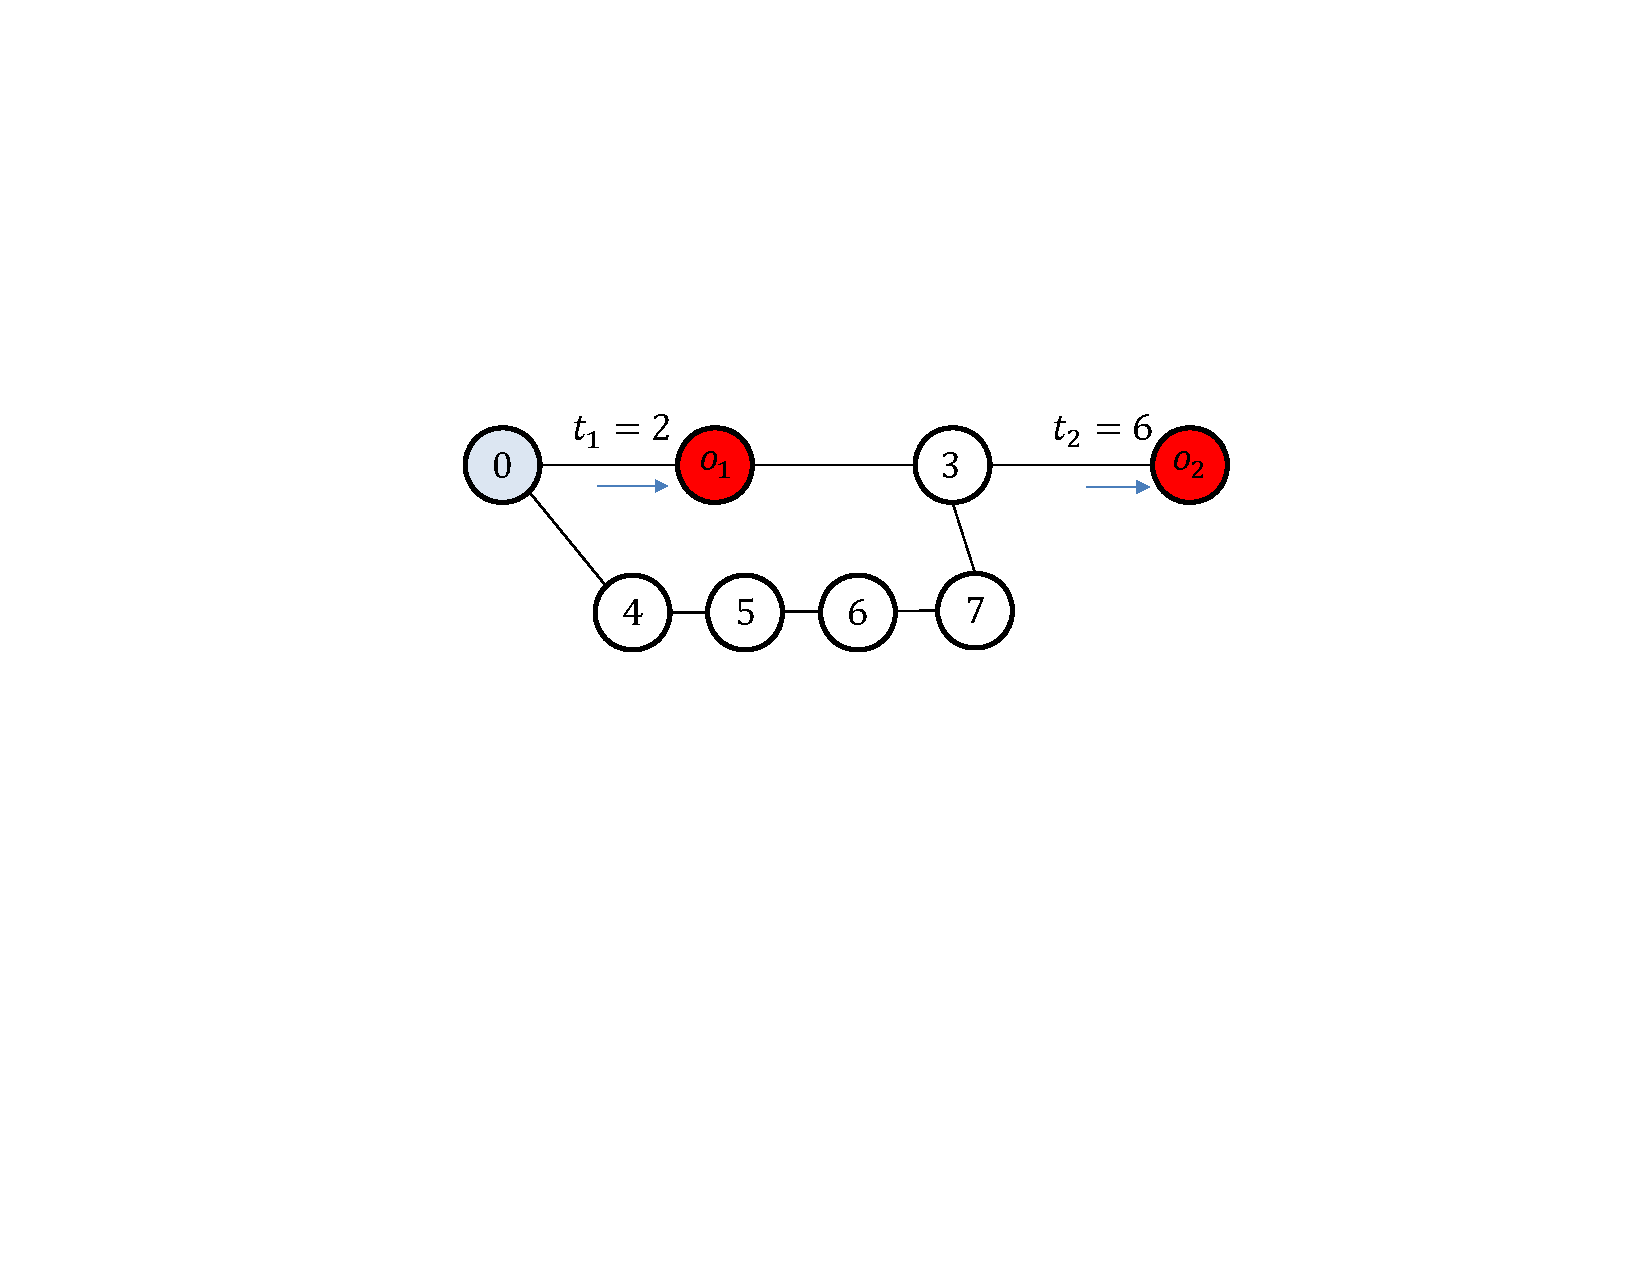
\includegraphics[width= 3in]{figures/pruning2}
\caption{The pruning used in \cite{pinto} can lead to false likelihood computations over loopy graphs; the scheme discounts the possibility of a spy passing the message to another spy.
%Delays $\theta_{ij}$ are modeled as Gaussians $\mathcal N(2,0.5)$, and spreading was run for 8 time units.
}
\label{fig:pruning2}
%\vspace*{-0.4in}
\end{figure}

\subsubsection{Trees}
We first tested the estimator on trees. As assumed in \cite{pinto}, each node transmits the message to its neighbors with an iid delay that is distributed according to $\mathcal N(2,0.5)$. Figure \ref{fig:pd_vs_spies} shows the probability of detection as a function of the fraction of spies over a 3-regular tree. We ran the simulation for 8 timesteps, leading to an average graph size of 75 nodes. Each datapoint is averaged over 4500 trials. Although \cite{pinto} does not provide simulation results over trees, we observe high detection probabilities for relatively low fractions of spies; with only 5 percent of the nodes spying, the source gets caught with probability 0.3. Note also that the ML estimator performs equally well with or without pruning (the plot lines are jittered to show both); this is because over trees, pruning never removes feasible candidates nodes or edges. We will see later that pruning over loopy graphs can remove feasible edges, and thereby impact the probability of detection. 
For reference, Figure \ref{fig:pd_vs_spies} also shows the probability of detection by the first-spy estimator. The ML estimator clearly outperforms the first-spy estimator, which is a good sanity check. Moreover, the first-spy estimator with pruning closely follows the theoretically-expected probability of detection; for a fraction of spies $p$, this probability grows as $P(\hat v=v^*)=1-(1-p)^d$ where $d$ denotes the degree of the underlying tree.
Figure \ref{fig:hops_vs_spies} shows the corresponding hop distances between the estimated source and the true source. We observe that with as few as 30 percent spies, this average hop distance is less than 0.1; the diameter of the graph is 8 hops. 
\begin{figure}
\centering
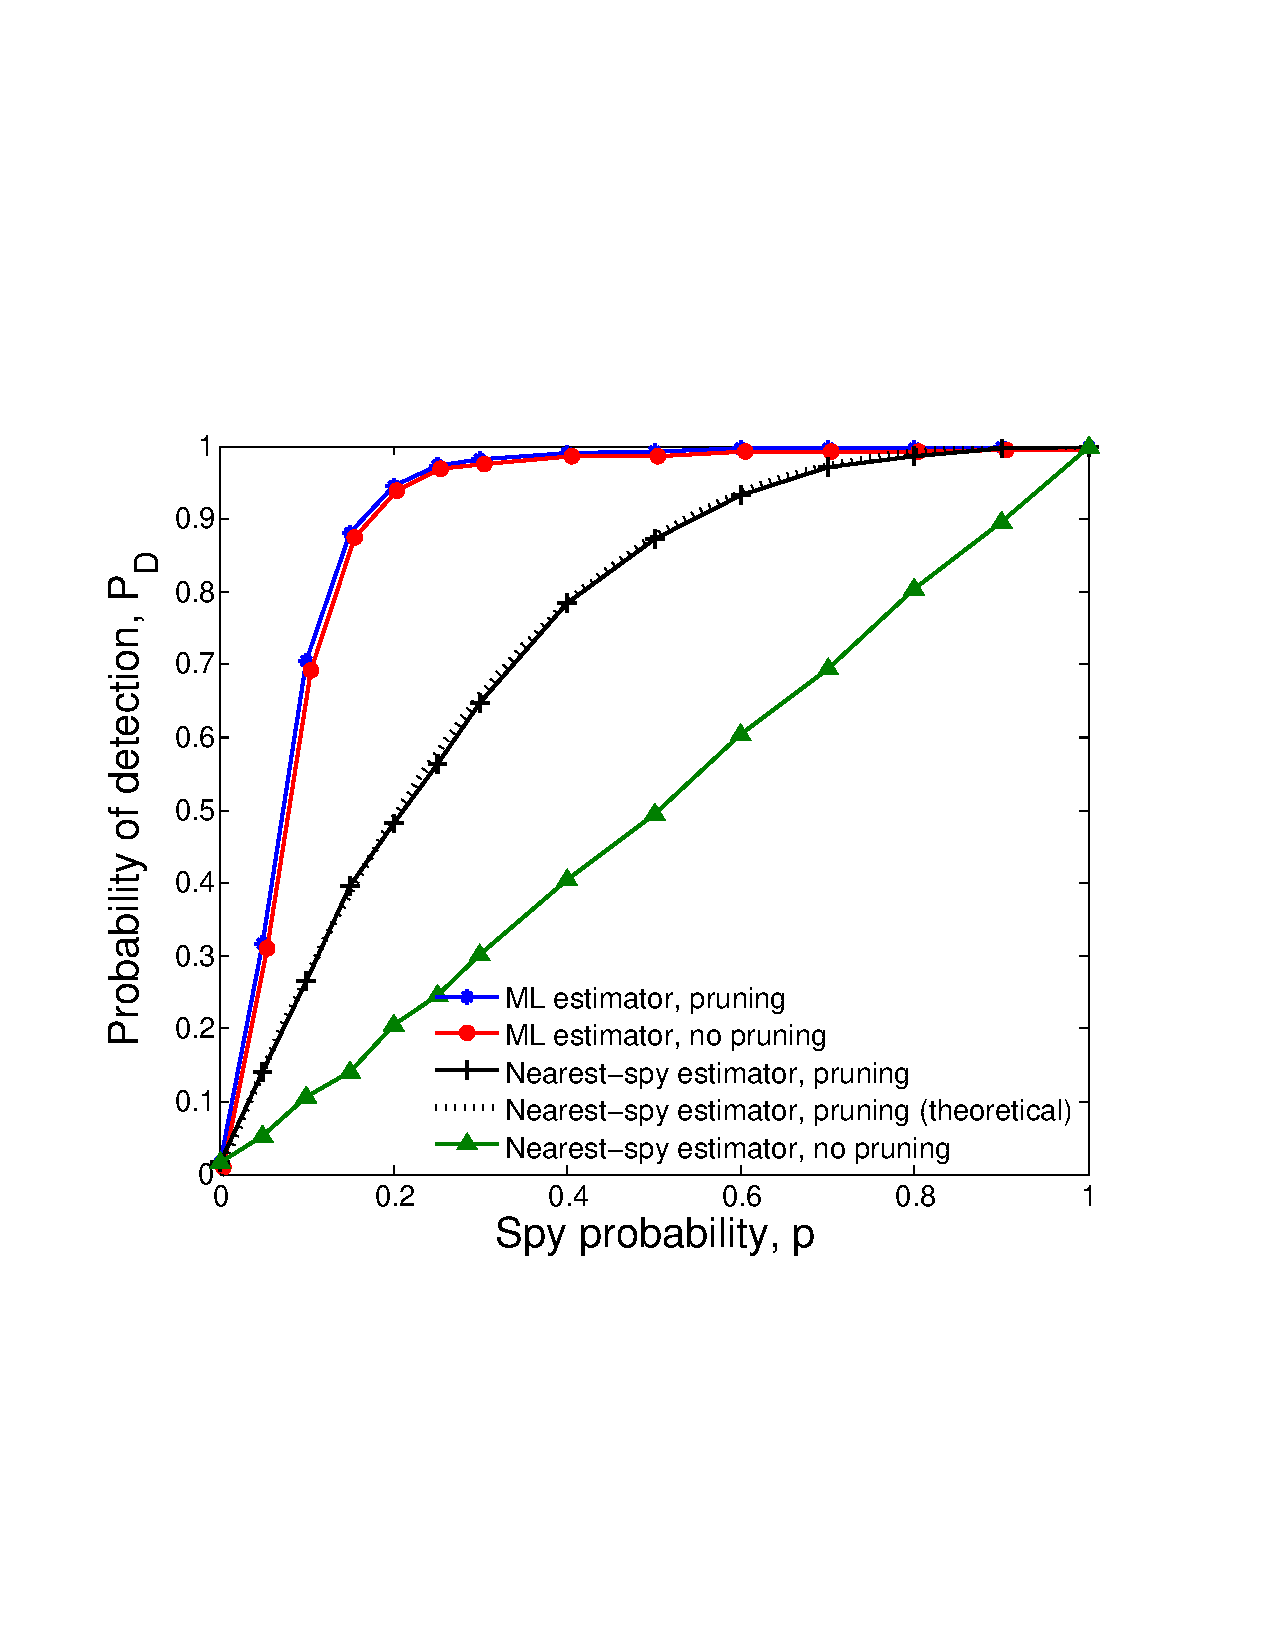
\includegraphics[height = 2.4in]{figures/pd_vs_spies}
\caption{Probability of detection, i.e. $P(\hat v = v^*)$, as a function of the spy probability $p$. This plot was generated over 3-regular trees. %Delays $\theta_{ij}$ are modeled as Gaussians $\mathcal N(2,0.5)$, and spreading was run for 8 time units.
}
\label{fig:pd_vs_spies}
%\vspace*{-0.4in}
\end{figure}

\begin{figure}
\centering
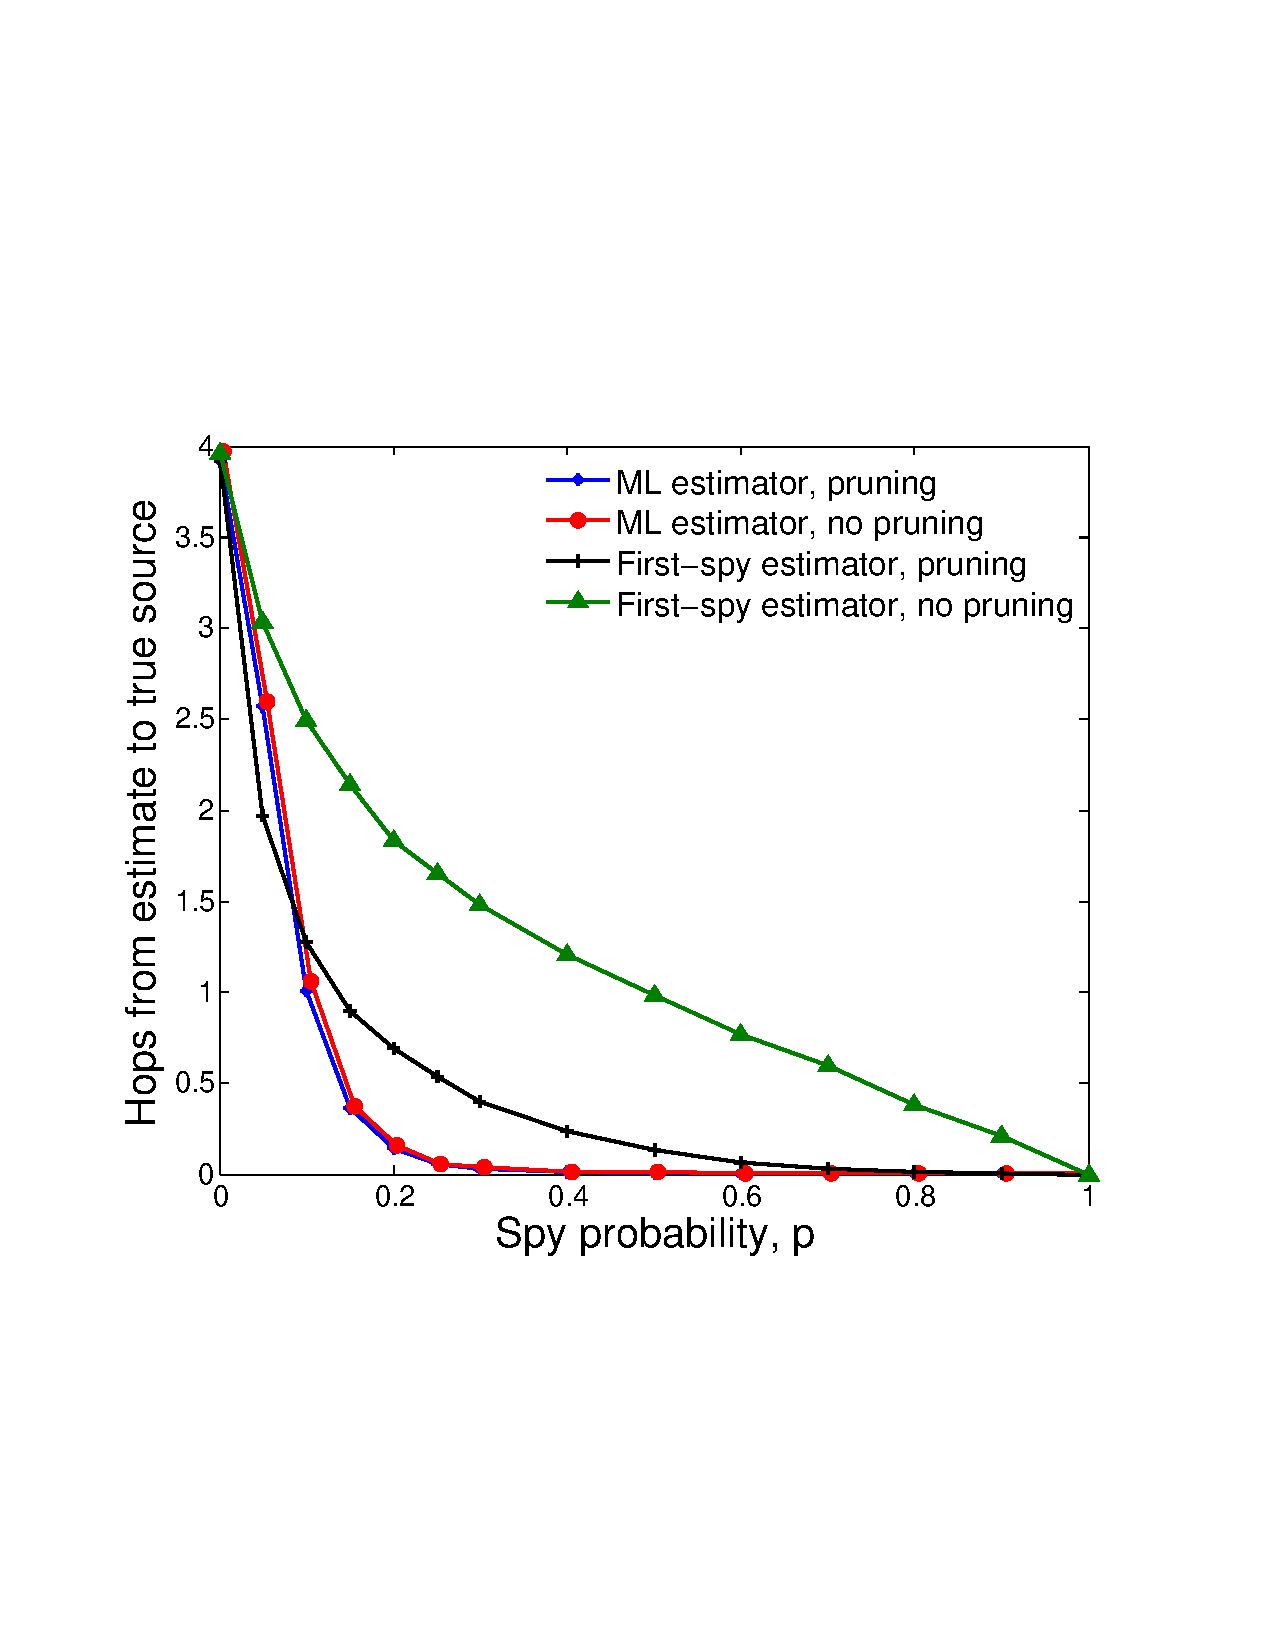
\includegraphics[height = 2.4in]{figures/hops_vs_spies}
\caption{Hop distance of the estimate $\hat v$ from the true source $v^*$ as a function of the spy probability $p$. This plot was generated over 3-regular trees. %Delays $\theta_{ij}$ are modeled as Gaussians $\mathcal N(2,0.5)$, and spreading was run for 8 time units.
}
\label{fig:hops_vs_spies}
%\vspace*{-0.4in}
\end{figure}

\subsection{Barabasi-Albert graphs}
We next considered random graphs with loops. \cite{pinto} considers a number of random graph structures, including Apollonian, Erdos-Renyi, and Barabasi-Albert. Due to time constraints, we only considered the latter. However, as mentioned earlier, we did not have access to the parameters used to generate the graphs in \cite{pinto}. To verify that we computed the estimator correctly, we considered a range of different parameters, and show that our results are at least plausibly consistent with the results provided in \cite{pinto}.

Figures \ref{fig:ba_graph} and \ref{fig:ba_graph_p1} show the probability of detection as a function of the fraction of spies for Barabasi-Albert graphs with $N=100$ nodes. We considered a minimum degree $m$ of 1 and 5. Each datapoint is averaged over 2000 trials. The figures illustrate that our numbers are at least plausible given the measurement provided in \cite{pinto}, albeit slightly low. We believe that over graphs with a higher minimum degree (e.g., $m=6$), the optimal estimator could reach 90 percent accuracy with 41 percent spies. Given the estimator's strong performance on trees, we believe that our estimator implementation is consistent with that in \cite{pinto}. %It also gives the right numbers when we compute the likelihoods for small graphs by hand. 

Note that the first-spy estimator with pruning performs as well or better than the `ML' estimator (which is not actually ML over general graph structures). Moreover, by plotting the pruned graph $\mathcal G_a$, we observed that $\mathcal G_a$ generally has very few honest nodes (about 10) when the fraction of spies is about 40; the pruned graph size decreases with spy fraction. 
We want to highlight that the first-spy estimator with pruning always returns a node from $\mathcal G_a$ by construction.  Moreover, the first-spy estimator achieves comparable accuracy to the ML estimator with orders of magnitude less computation; the first-spy estimator has complexity $O(1)$ as compared to $O(N^3)$ for the ML estimator. As such, one of the main takeaways from our study is that when direction-of-infection information is available and the graph not tree-structured, there is no reason to use the estimator from \cite{pinto}; the first-spy estimator will do as well or better, while using only a fraction of the computation. 

Conversely, when there is no direction-of-infection information, the first-spy estimator performs quite poorly compared the estimator from \cite{pinto}. Even the hop distances, illustrated in Figures \ref{fig:ba_hops} and \ref{fig:ba_hops_p1}, are significantly higher than the other tested estimators for the first-spy estimator without pruning. As such, the Pinto \emph{et al.} estimator may be quite powerful when there is no direction information available; this problem setting was not explored in their original paper.

\begin{figure*}[ht] \label{ fig7} 
  \begin{minipage}[b]{0.48\linewidth}
    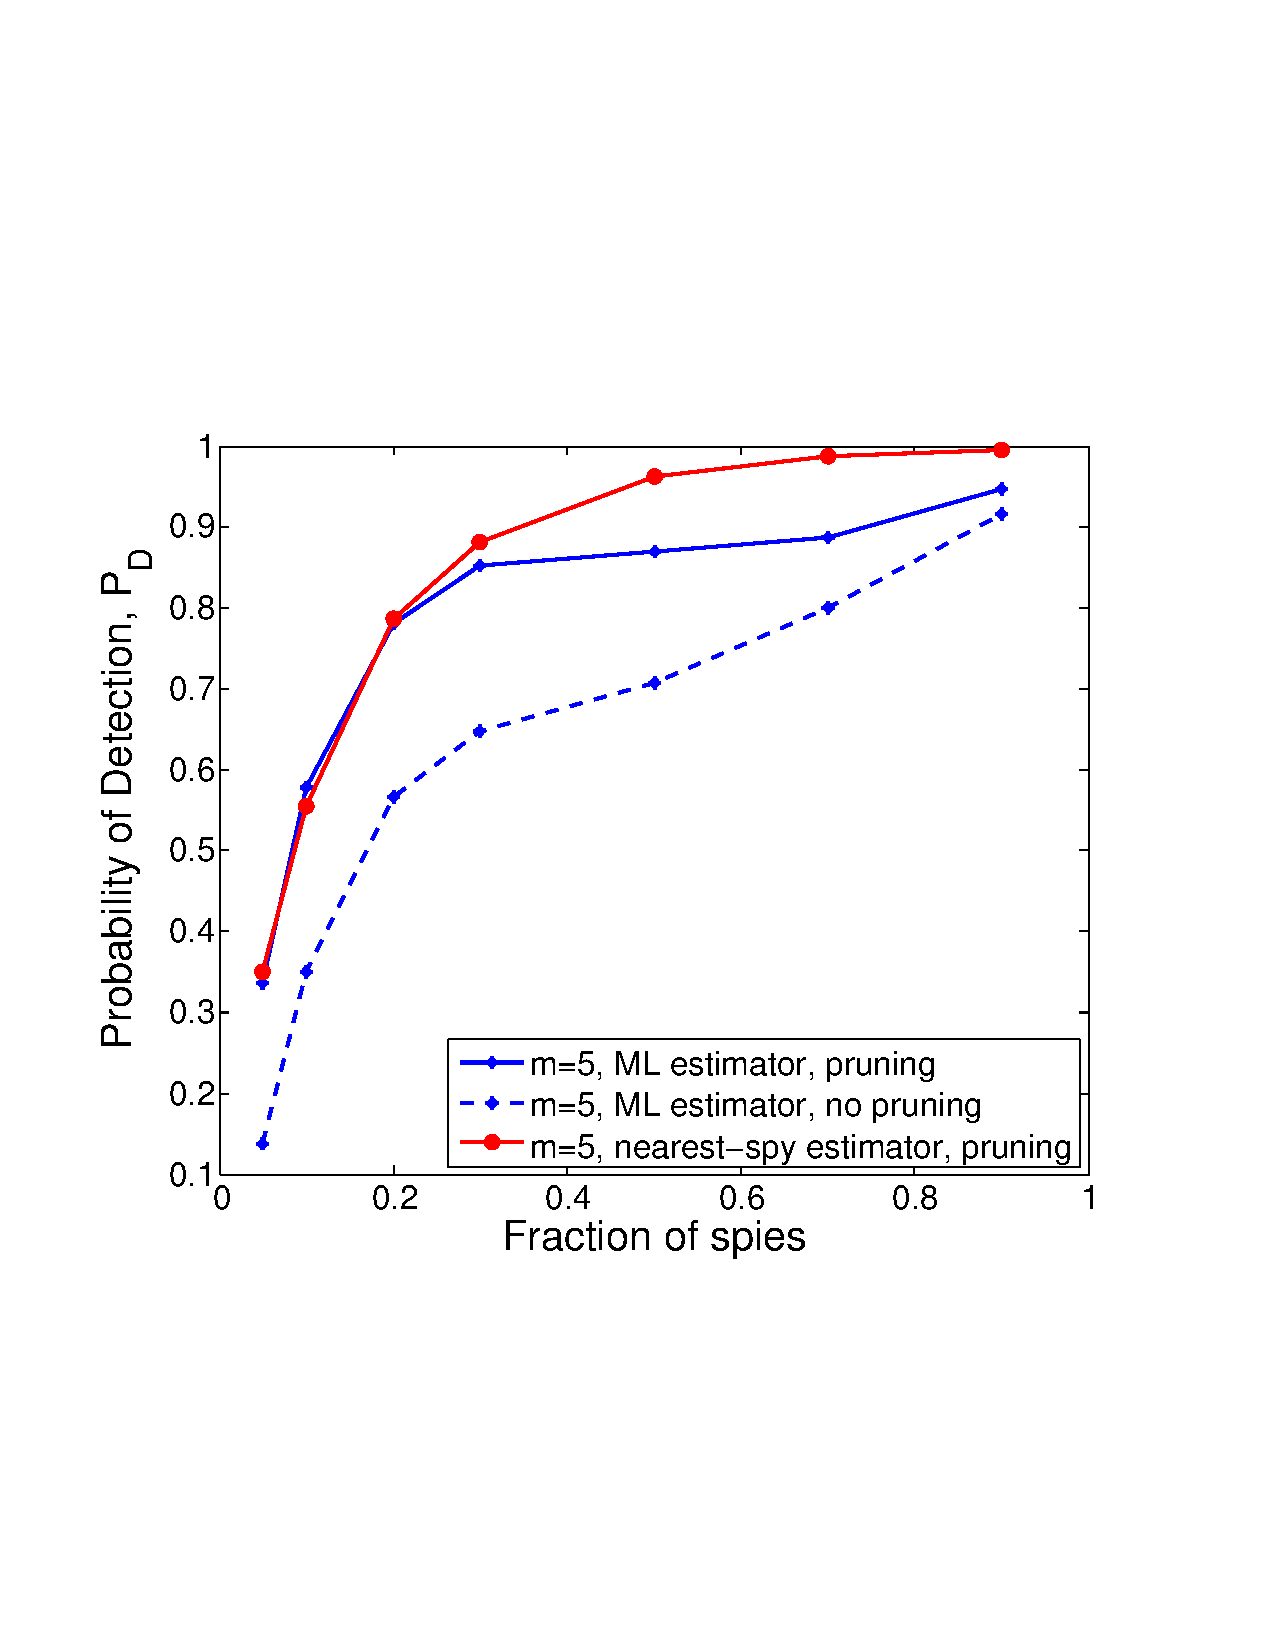
\includegraphics[width=3in]{figures/ba_graphs} 
    \caption{Probability of detection vs. spy fraction over Barabasi-Albert graphs with minimum degree $m=5$ and number of nodes $N=100$.} 
\label{fig:ba_graph}
  \end{minipage} 
\begin{minipage}[b]{0.48\linewidth}
    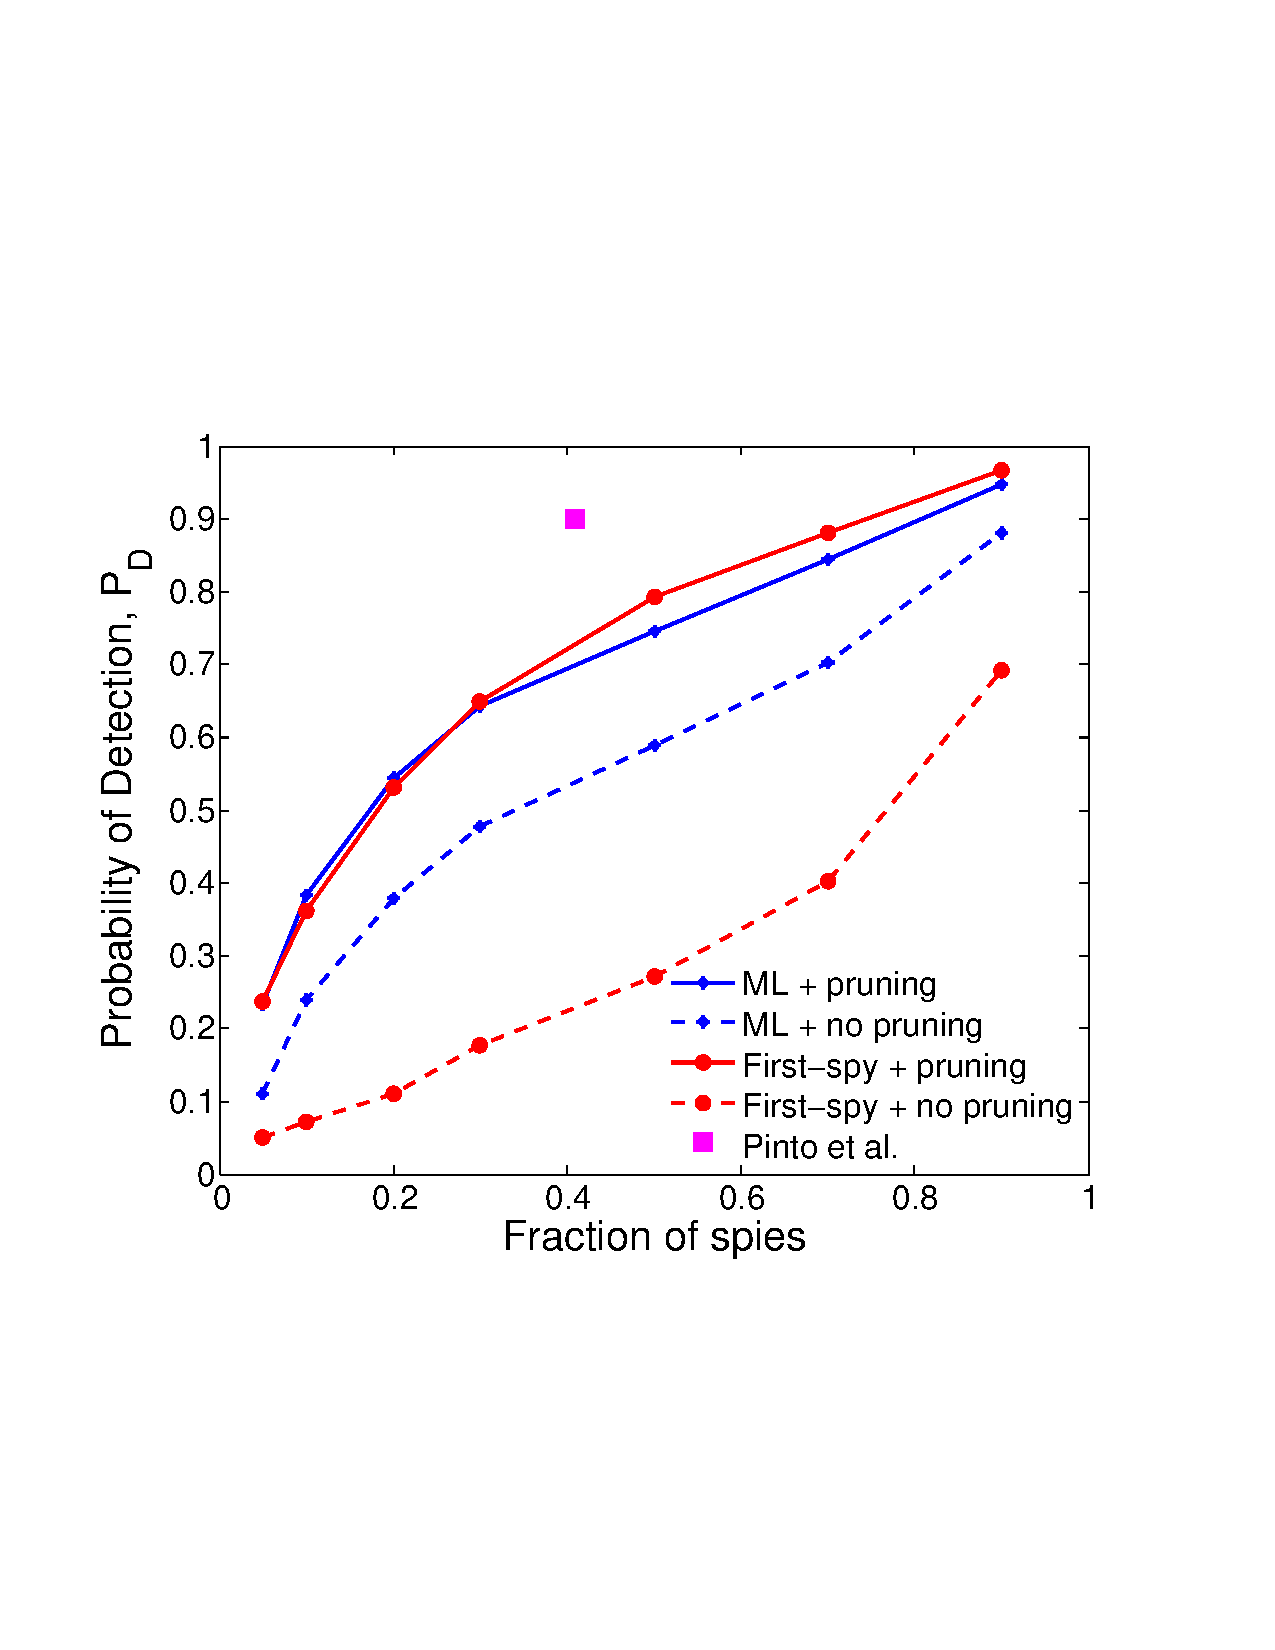
\includegraphics[width=3in]{figures/ba_graphs_p1} 
    \caption{Probability of detection vs. fraction over Barabasi-Albert graphs with minimum degree $m=1$ and number of nodes $N=100$.} 
\label{fig:ba_graph_p1}
  \end{minipage}
  \begin{minipage}[b]{0.48\linewidth}
    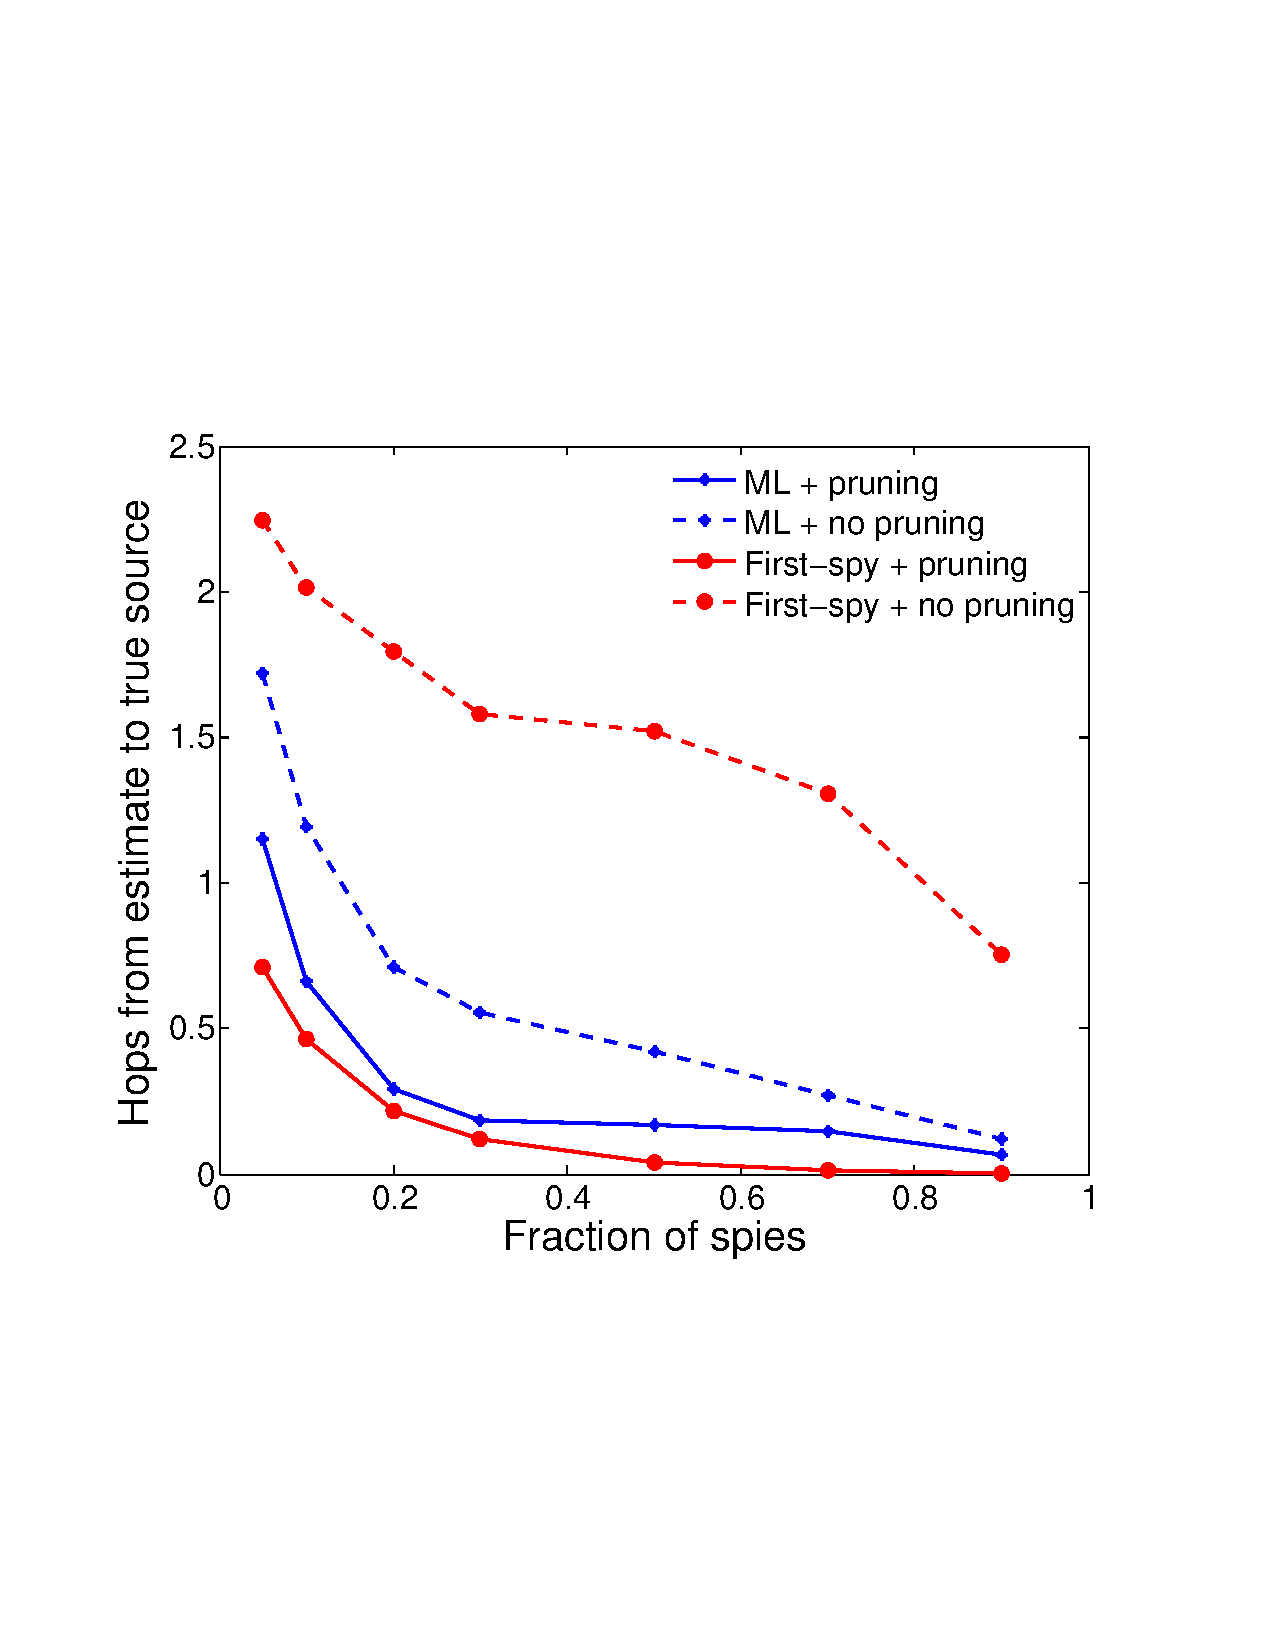
\includegraphics[width=3in]{figures/ba_hops} 
    \caption{Hop distance from estimate to true source vs. spy fraction over Barabasi-Albert graphs with minimum degree $m=5$ and number of nodes $N=100$.} 
\label{fig:ba_hops}
  \end{minipage} 
  \hfill
  \begin{minipage}[b]{0.48\linewidth}
    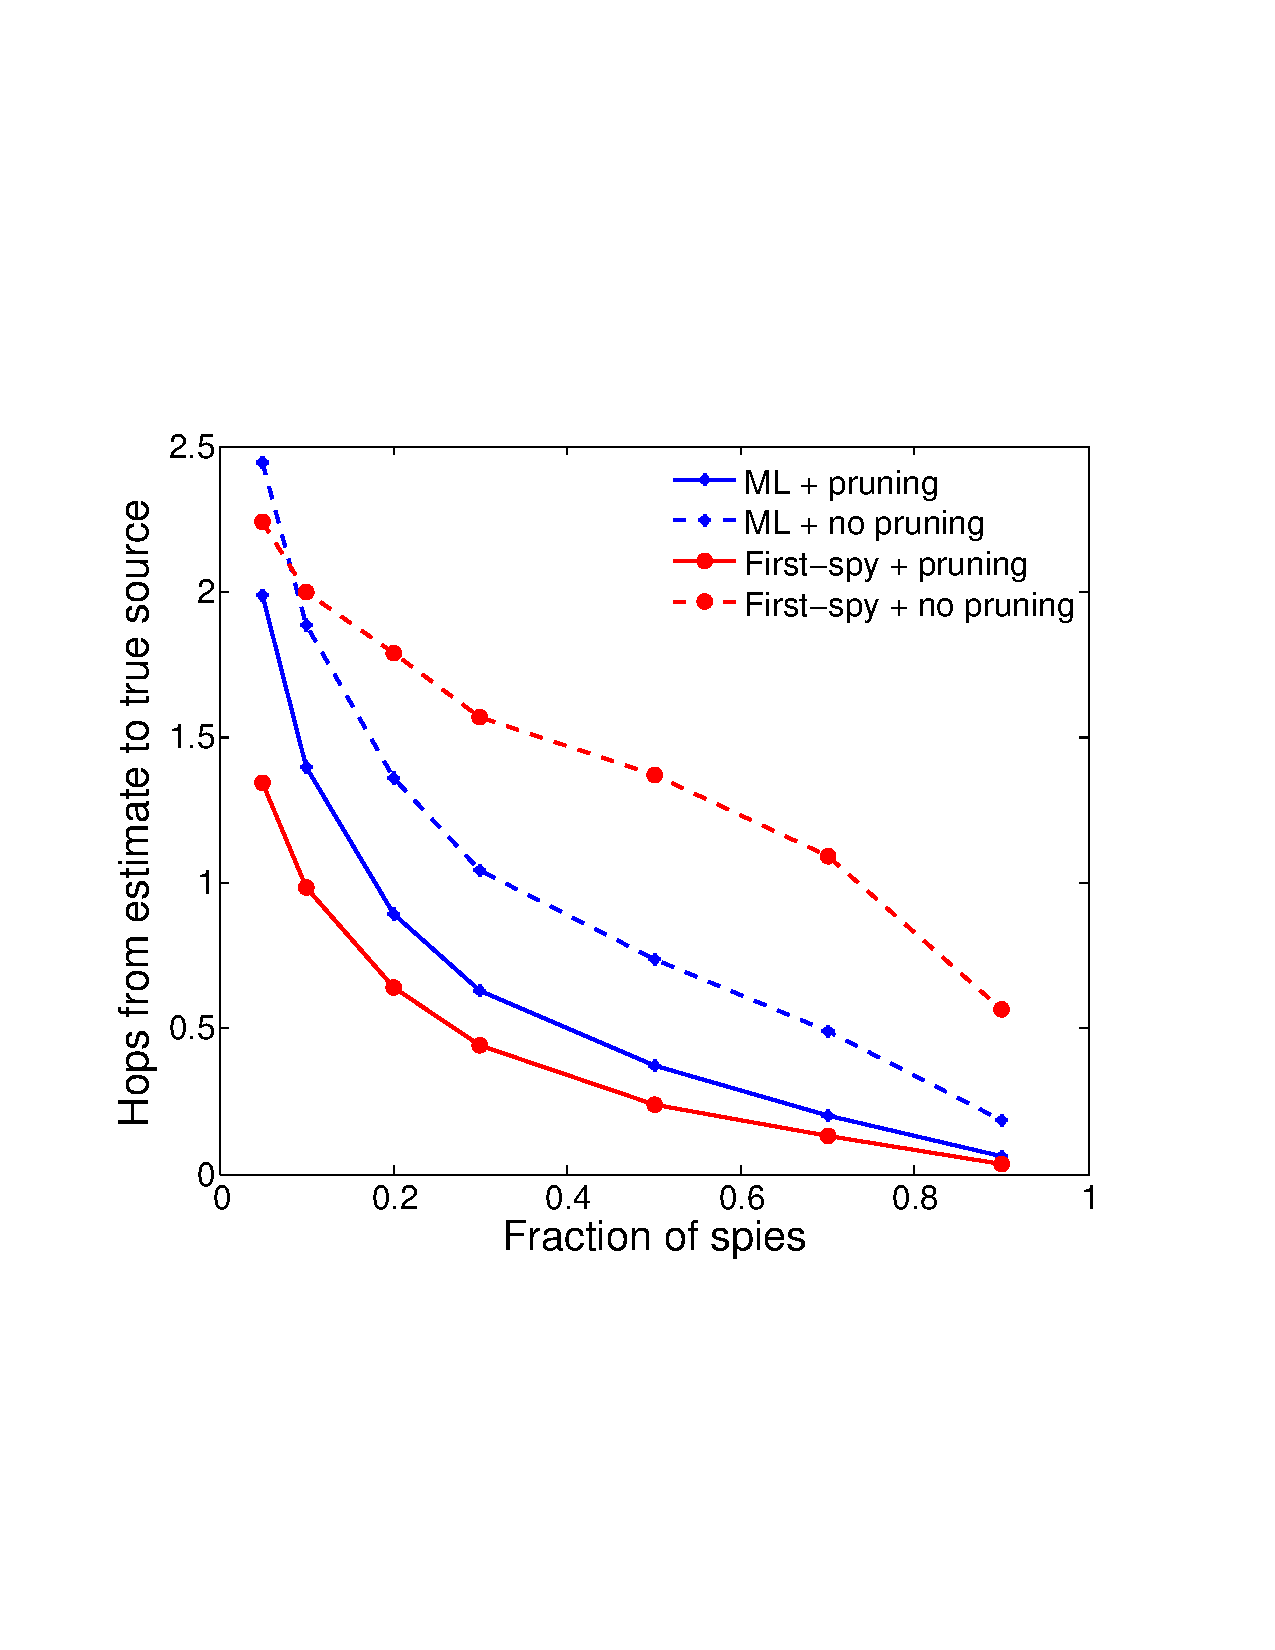
\includegraphics[width=3in]{figures/ba_hops_p1} 
    \caption{Hop distance from estimate to true source vs. spy fraction over Barabasi-Albert graphs with minimum degree $m=1$ and number of nodes $N=100$.} 
  \end{minipage} 
\label{fig:ba_hops_p1}
\end{figure*}


\subsection{Facebook dataset}

Randomized graphs provide decent estimates for the estimators' effectivness, but they are still different from real datasets. In order to test our estimators on realistic data, we use a Facebook dataset~\cite{viswanath-2009-activity} from New Orleans. The dataset contains all of the user-to-user connections on Facebook in New Orleans. Since the number of users is large, we use \emph{ego sampling} on the dataset. Ego sampling takes a random node from the graph and samples all nodes within $n$ hops from the initial node. For our experiments, we use $n = 2$.
